
\documentclass[12pt]{article}
\usepackage{amsmath}
\usepackage{graphicx}
\usepackage{geometry}
\usepackage[applemac]{inputenc}

\geometry{left=1in,right=1in,top=1in,bottom=1in}


% first colour for latex or pdflatex
\ifx\pdfoutput\@undefined\usepackage[usenames,dvips]{color}
\else\usepackage[usenames,dvipsnames]{color}
% and fix pdf colour problems
\IfFileExists{pdfcolmk.sty}{\usepackage{pdfcolmk}}{} 
\fi
% second test for a5paper
%\ifdim\paperwidth=148mm \usepackage[a5paper]{geometry}\fi
% lastly load colour hyperref
\usepackage[plainpages=false,pdfpagelabels,pagebackref=false,naturalnames=true,hyperindex=true,pdftitle={***}]{hyperref}
\hypersetup{colorlinks=true,
urlcolor=Cerulean,linkcolor=BrickRed,citecolor=RoyalBlue,
  pdfpagemode=None,
  pdfstartview=FitH}
\usepackage[all]{hypcap}

\begin{document}

\title{Language statistics at different temporal, geographical, and grammatical scales}
%\author{Carlos Gershenson$^{1,2,3}$ \\
%$^{1}$ Departamento de Ciencias de la Computaci\'on\\
%Instituto de Investigaciones en Matem\'aticas Aplicadas y en Sistemas \\
%Universidad Nacional Aut\'onoma de M\'exico\\
%A.P. 20-726, 01000 M\'exico CDMX M\'exico\\
%\href{mailto:cgg@unam.mx}{cgg@unam.mx} \
%\url{http://turing.iimas.unam.mx/~cgg} \\
%$^{2}$ Centro de Ciencias de la Complejidad \\
%Universidad Nacional Aut\'onoma de M\'exico\\
%$^{3}$ ITMO University, Russian Federation.}
\maketitle

\begin{abstract}
***
\end{abstract}

\section{Introduction}

The statistical study of languages is not new~\cite{zipf}, but recent data availability has allowed the possibility of analyzing how languages and their use has changed in time~\cite{Michel14012011,Perc07122012,PhysRevX.3.021006,Cocho2015}. 
These studies have considered language change during years and centuries. What can we say about change --- not so much of language itself, but of its use --- during hours and days? To address this question, we use geolocated Twitter data to compare languages at short timescales, at different spatial scales, and at different ``grammatical scales''.


\section{Methods and Data}

Explain rank diversity, include an illustrative spaghetti figure, including marks for $\Delta t$.
\cite{Cocho2015,Morales2016,10.3389/fphy.2018.00045,Cocho2019}
We have found that rank diversity curves for six different Indoeuropean languages are very similar, as they can be fitted with a sigmoid curve with small differences between languages. 

Explain data: how it was collected (Alfredo), papers where this data has been used \cite{Morales2014,doi:10.1063/1.4913758,doi:10.1098/rsif.2016.1048}

Data statistics (how many tweets/words/Ngrams), languages, how it was processed (to keep same number of tweets), etc.

Explain scales: temporal, geographical, grammatical. 

already studies of grammatical scale for Google Books \cite{10.3389/fphy.2018.00045}. We have found that the grammatical scale varies language statistics (rank diversity, change probability, rank entropy and rank complexity) more than changes of language. In other words, a change of grammatical scale implies a greater change in the statistics than a change of language.

\section{Results}

Explain figures

\begin{figure}[htbp]
\begin{center}
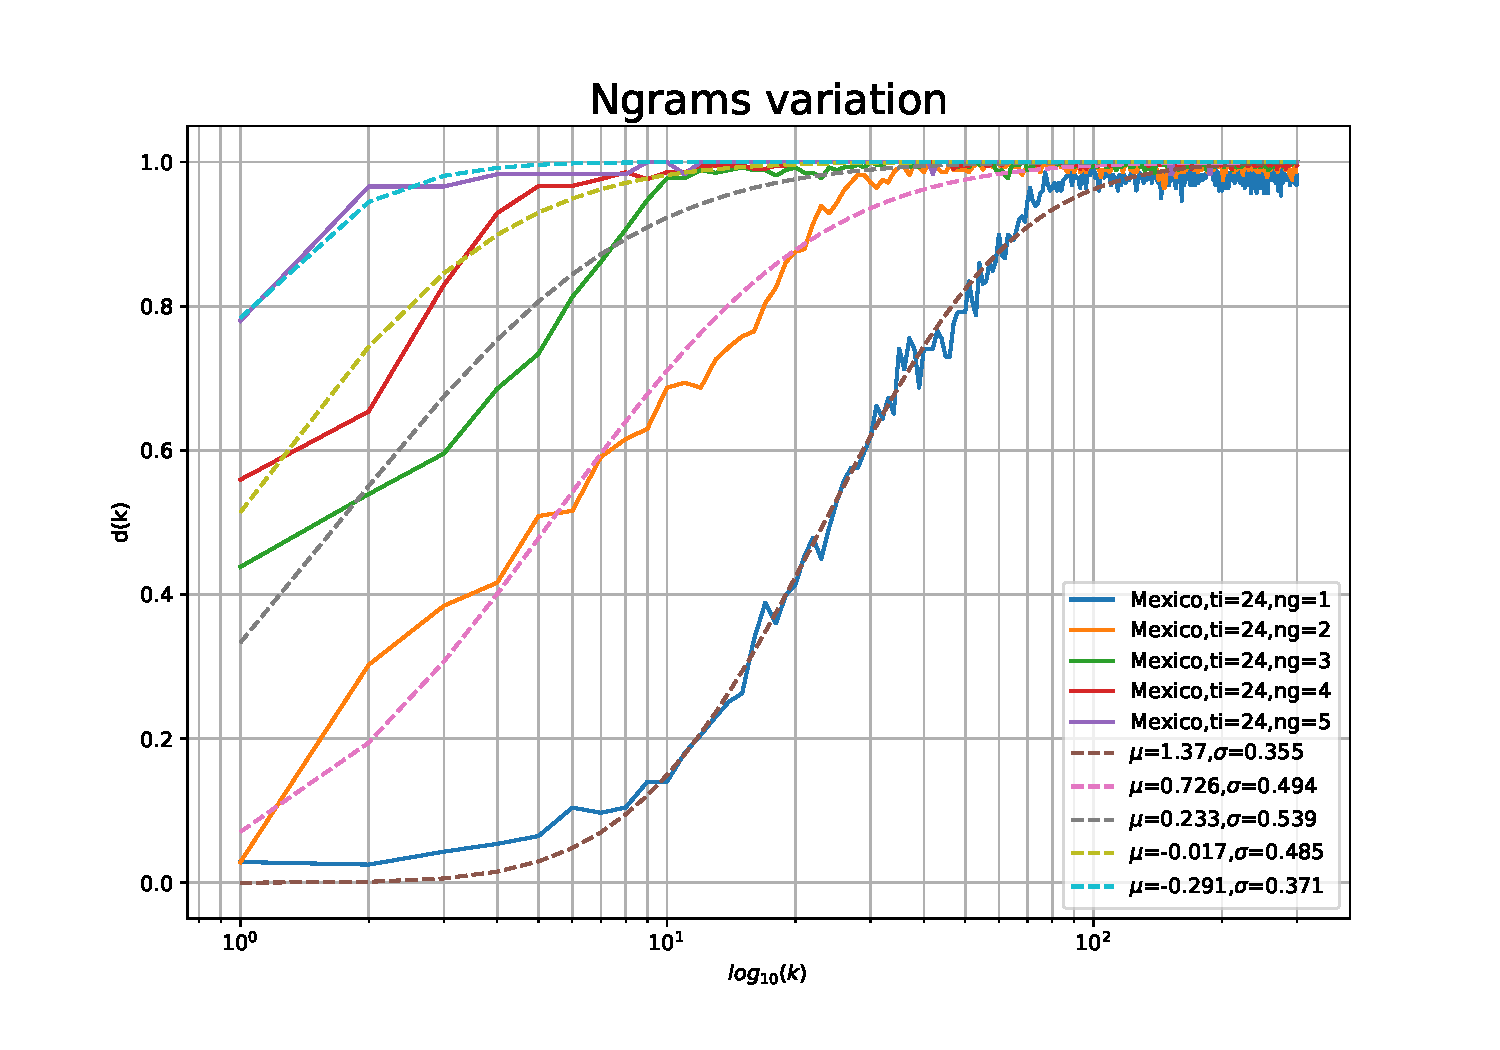
\includegraphics[width=0.9\textwidth]{img/N-Mexico}
\caption{Rank diversities from Mexico for different grammatical scales, $\Delta t = 24$hr.}
\label{fig:N-Mexico}
\end{center}
\end{figure}

\begin{figure}[htbp]
\begin{center}
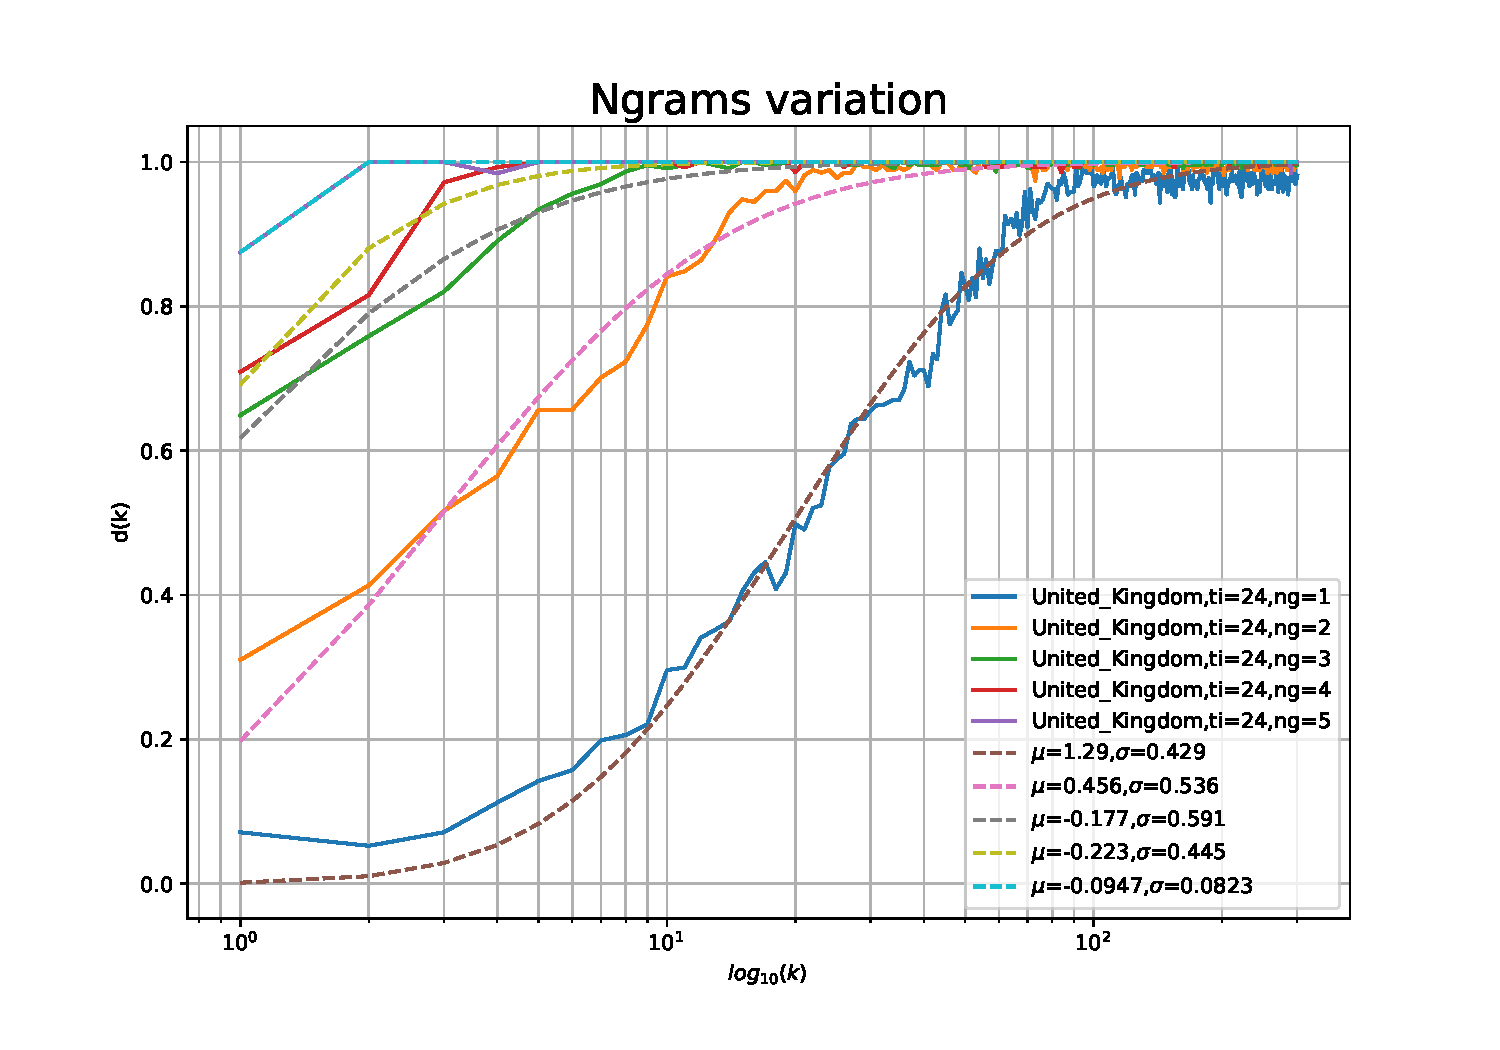
\includegraphics[width=0.9\textwidth]{img/N-United_Kingdom}
\caption{Rank diversities from the United Kingdom for different grammatical scales, $\Delta t = 24$hr.}
\label{fig:N-United_Kingdom}
\end{center}
\end{figure}

\begin{figure}[htbp]
\begin{center}
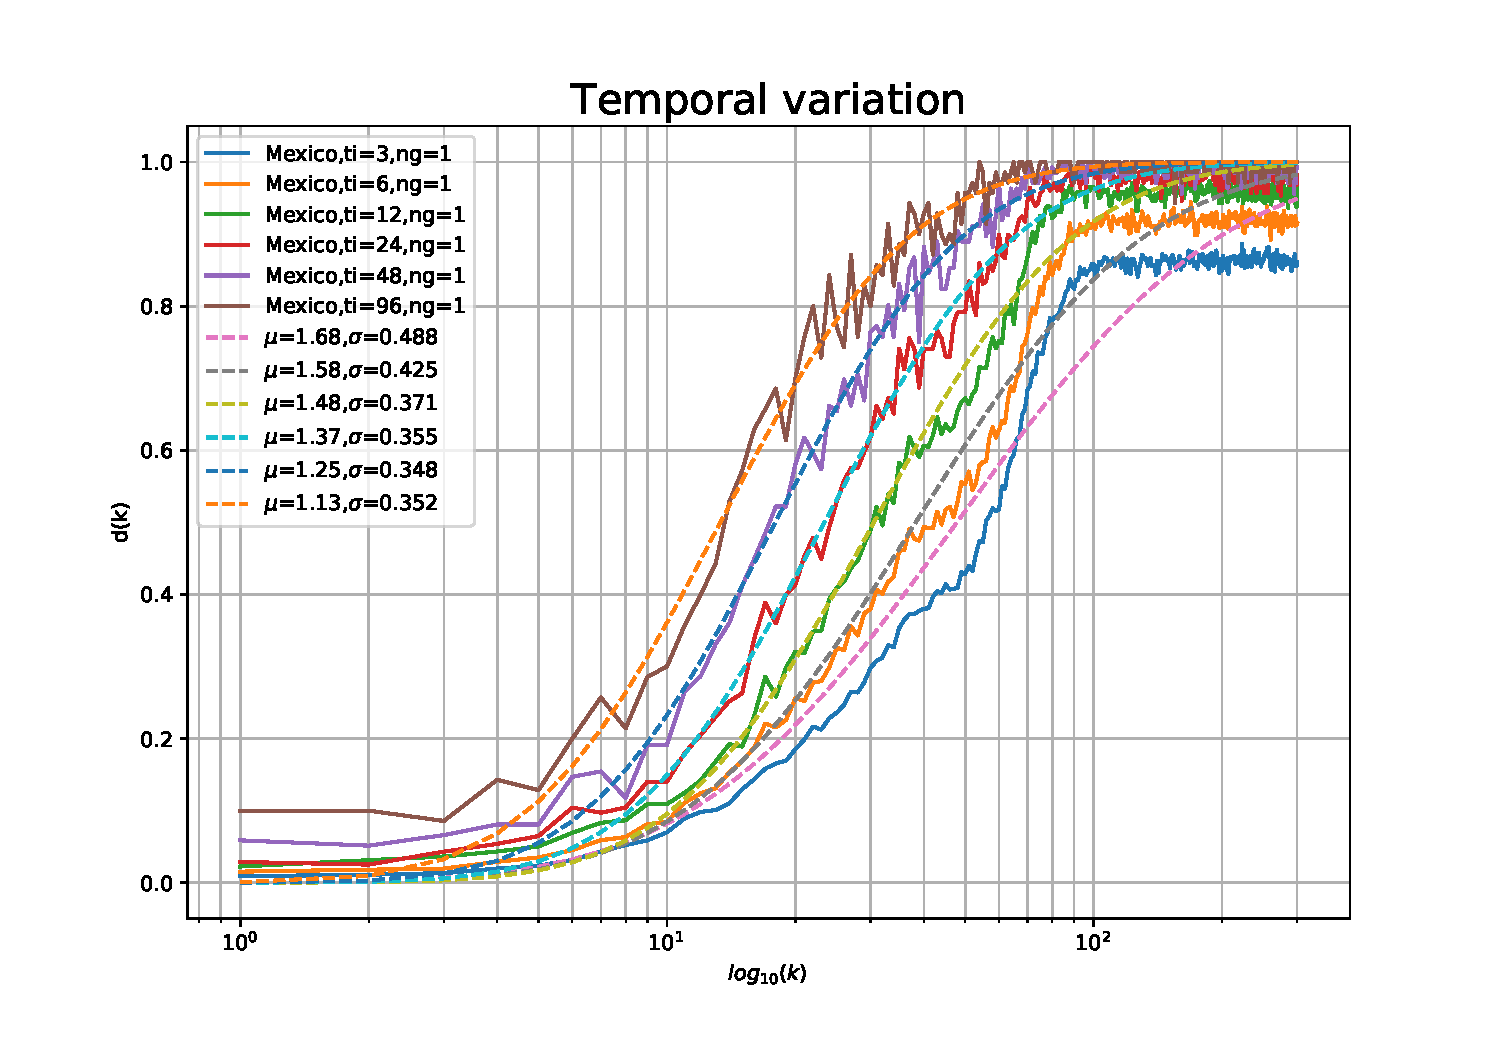
\includegraphics[width=0.9\textwidth]{img/time-Mexico}
\caption{Rank diversities from Mexico for different temporal scales, $N = 1$.}
\label{fig:time-Mexico}
\end{center}
\end{figure}

\begin{figure}[htbp]
\begin{center}
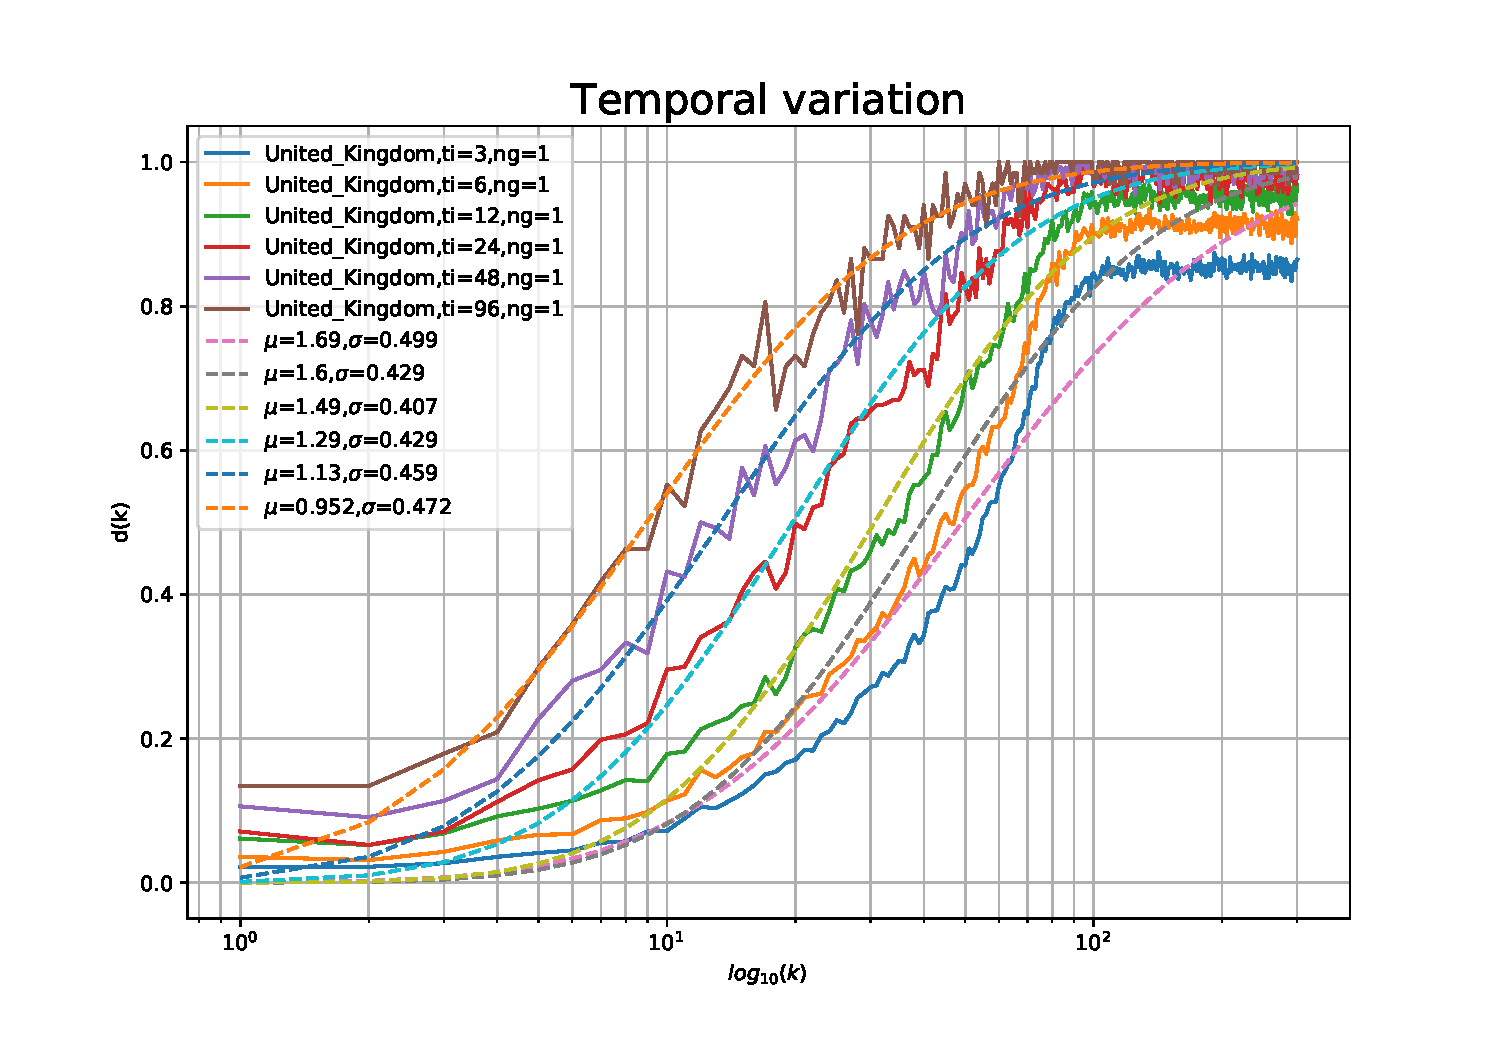
\includegraphics[width=0.9\textwidth]{img/time-United_Kingdom}
\caption{Rank diversities from the United Kingdom for different temporal scales, $N = 1$.}
\label{fig:time-United_Kingdom}
\end{center}
\end{figure}


\begin{figure}[htbp]
\begin{center}
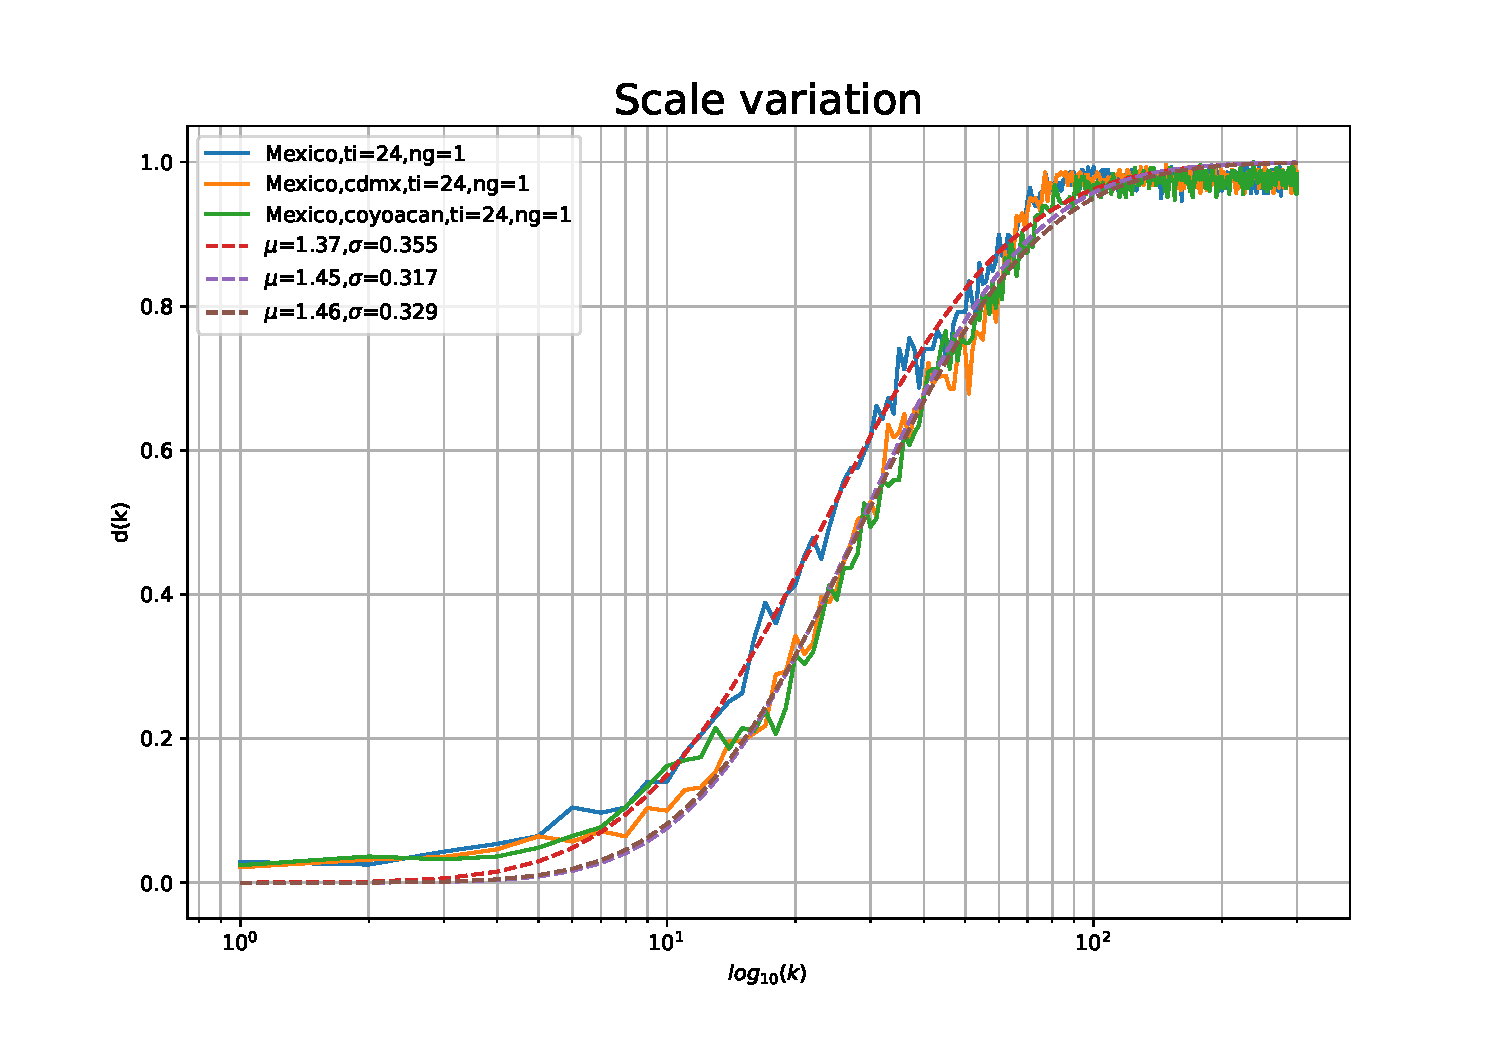
\includegraphics[width=0.9\textwidth]{img/geo-mx-24hrs}
\caption{Rank diversities from Mexico for different geographical scales, $N = 1$, $\Delta t = 24$hr.}
\label{fig:geo-mx-24hrs}
\end{center}
\end{figure}

\begin{figure}[htbp]
\begin{center}
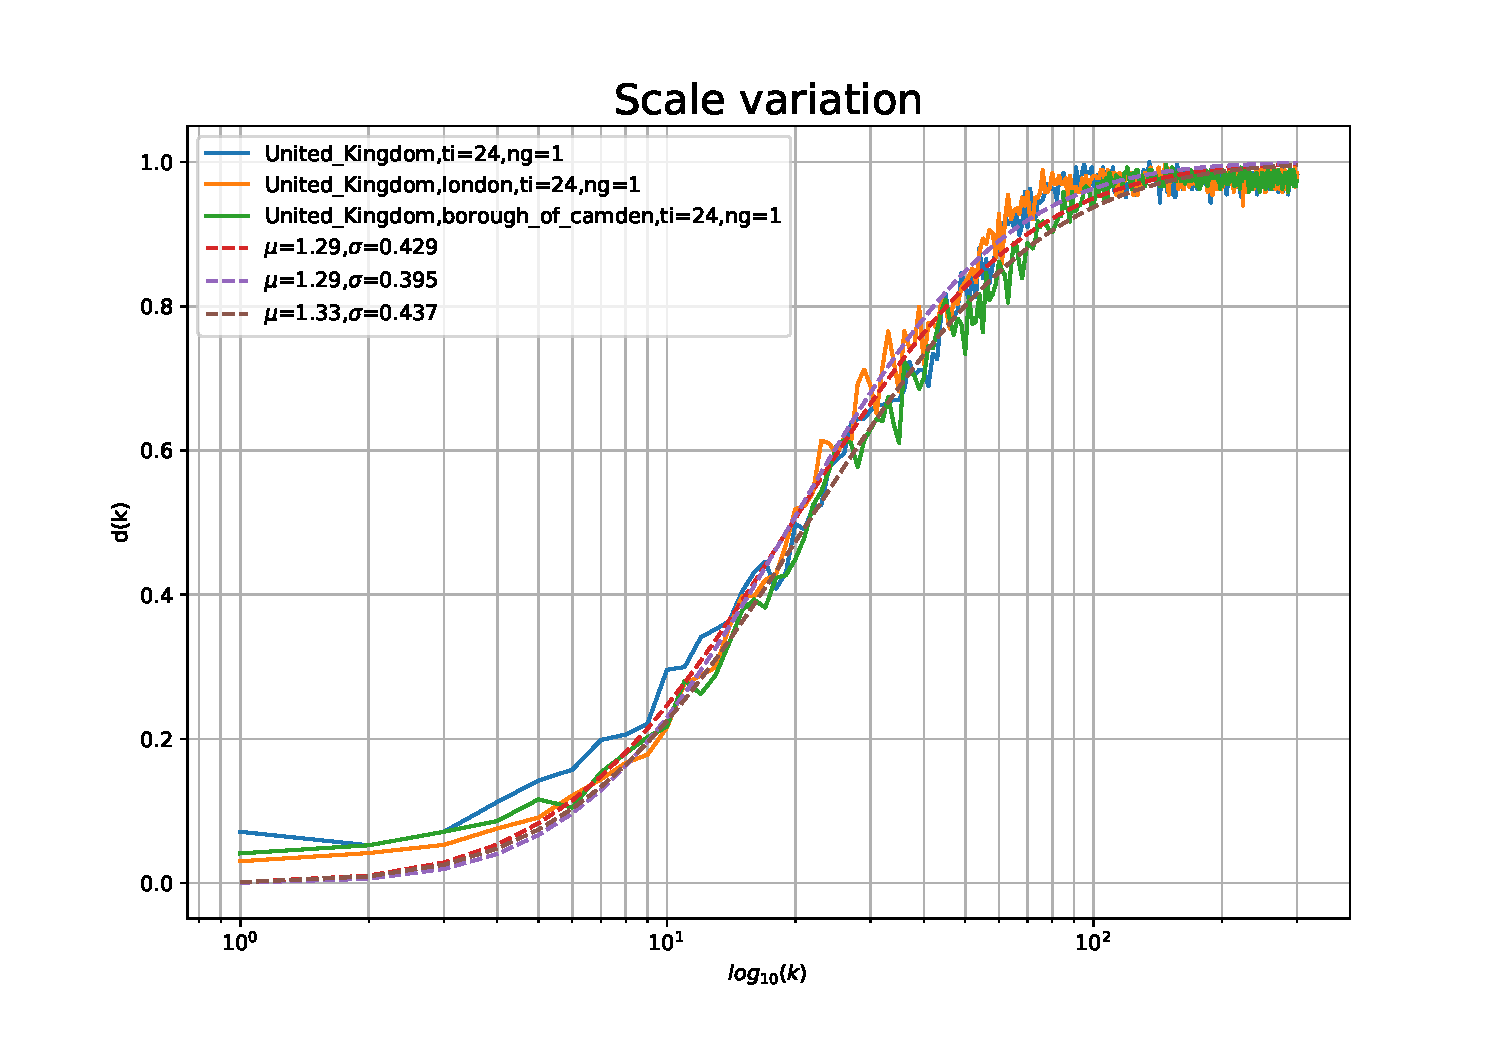
\includegraphics[width=0.9\textwidth]{img/geo-uk-24hrs}
\caption{Rank diversities from the United Kingdom for different geographical scales, $N = 1$, $\Delta t = 24$hr.}
\label{fig:geo-uk-24hrs}
\end{center}
\end{figure}





scales vs. $\mu$'s

\section{Conclusions}


Which scales are more relevant? All of them, but grammatical $>$ temporal $>$ geographical.
In general, rank diversity grows faster at higher scales in all three cases.

\section*{Acknowledgments}

%We should like to\ thank ***. 
%This work was partially supported by SNI membership 47907 of CONACyT, Mexico. 

\bibliographystyle{unsrt}
\bibliography{carlos,refs}


\end{document}
